  \section[OpenStack]{OpenStack : le projet, utilisation du IaaS}

  \subsection[OpenStack le projet]{Présentation du projet}

  \begin{frame}
    \frametitle{Vue haut niveau}
    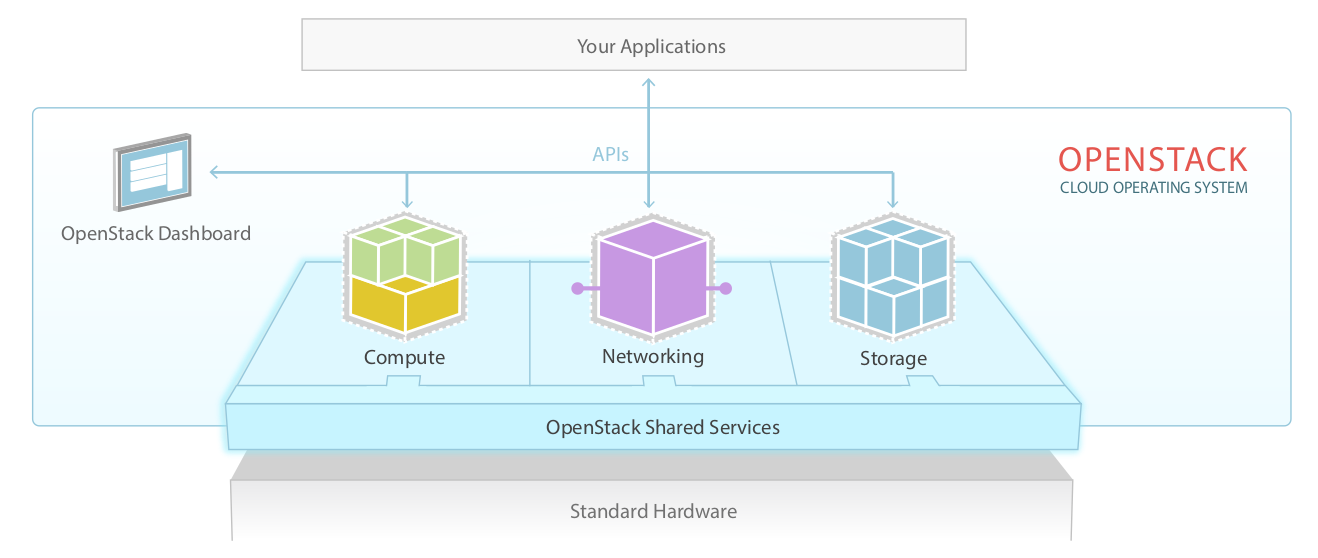
\includegraphics[width=\textwidth]{images/openstack-software-diagram.pdf}
  \end{frame}

  \begin{frame}
    \frametitle{Historique}
    \begin{itemize}
      \item Démarrage en 2010
      \item Objectif : le Cloud Operating System libre
      \item Fusion de deux projets de Rackspace (Storage) et de la NASA (Compute)
      \item Logiciel libre distribué sous licence Apache 2.0\pause
      \item Les releases jusqu'à aujourd'hui :
      \begin{itemize}
        \item Austin (2010.1)
        \item Bexar (2011.1)
        \item Cactus (2011.2)
        \item Diablo (2011.3)
        \item Essex (2012.1)
        \item Folsom (2012.2)
        \item Grizzly (2013.1)
        \item Havana (2013.2)
        \item Icehouse (2014.1)
        \item Juno (2014.2)
        \item Kilo (2015.1)
        \item \textbf{Liberty (2015.2)}\pause
        \item Avril 2016 : Mitaka
      \end{itemize}
    \end{itemize}
  \end{frame}

  \begin{frame}
    \frametitle{Statistiques : Kilo}
    \begin{itemize}
      \item 1492 contributeurs (Liberty : 1933)
      \item 169 organisations
      \item 394 nouvelles fonctionnalités et 7257 bugs corrigés
      \item 113 drivers/plugins
      \item 792200 chaines traduites
    \end{itemize}
    Source : \url{http://lists.openstack.org/pipermail/foundation-board/2015-April/000050.html}
  \end{frame}

  \begin{frame}
    \frametitle{Quelques soutiens/contributeurs ...}
    \begin{itemize}
      \item \textcolor{blue}{Rackspace} et la NASA\pause
      \item \textcolor{blue}{Canonical}
      \item \textcolor{blue}{Red Hat}
      \item \textcolor{blue}{SUSE}\pause
      \item \textcolor{blue}{HP}
      \item \textcolor{blue}{IBM}
      \item \textcolor{cyan}{Dell}, \textcolor{cyan}{Intel}
      \item \textcolor{cyan}{Cisco}, \textcolor{cyan}{Juniper}\pause
      \item \textcolor{cyan}{NetApp}, VMWare\pause
      \item \textcolor{cyan}{Yahoo}, Bull\pause
      \item Mais aussi : \textcolor{cyan}{Mirantis}, eNovance (racheté par Red Hat), \textcolor{cyan}{DreamHost}, Hastexo, StackOps\pause
      \item et \textbf{Google} ! (depuis juillet 2015)
    \end{itemize}
    \url{http://www.openstack.org/foundation/companies/}
  \end{frame}

  \begin{frame}
    \frametitle{... et utilisateurs}
    \begin{itemize}
      \item Tous les contributeurs précédemment cités\pause
      \item En France : \textbf{Cloudwatt} et \textbf{Numergy}\pause
      \item Wikimedia
      \item CERN
      \item Paypal
      \item Comcast
      \item BMW\pause
      \item Etc. Sans compter les implémentations confidentielles
    \end{itemize}
    \url{http://www.openstack.org/user-stories/}
  \end{frame}

  \begin{frame}
    \frametitle{Les différents sous-projets}
    \begin{itemize}
        \item OpenStack Compute - Nova
        \item OpenStack (Object) Storage - Swift\pause
        \item OpenStack Block Storage - Cinder\pause
        \item OpenStack Networking - Neutron\pause
        \item OpenStack Image Service - Glance\pause
        \item OpenStack Identity Service - Keystone\pause
        \item OpenStack Dashboard - Horizon\pause
        \item OpenStack Telemetry - Ceilometer\pause
        \item OpenStack Orchestration - Heat\pause
        \item OpenStack Database Service - Trove
    \end{itemize}
  \end{frame}

  \begin{frame}
    \frametitle{Les différents sous-projets (2)}
    \begin{itemize}
      \item Mais aussi :
      \begin{itemize}
        \item Bare metal (Ironic)
        \item Queue service (Zaqar)
        \item Data processing (Sahara)
        \item DNS service (Designate)
        \item Shared File Systems (Manila)
        \item Key management (Barbican)
        \item PaaS (Solum)\pause
        \item Container (Magnum)
      \end{itemize}\pause
      \item Autres
      \begin{itemize}
        \item Les clients (python-*client)
      \end{itemize}
    \end{itemize}
  \end{frame}

  \begin{frame}
    \frametitle{Développement du projet : les principes}
    \begin{itemize}
      \item Open Source
      \item Open Design
      \item Open Development
      \item Open Community
    \end{itemize}
  \end{frame}

  \begin{frame}
    \frametitle{La fondation OpenStack}
    \begin{itemize}
      \item Entité de gouvernance principale du projet
      \item Représentation juridique du projet
      \item Les membres du board sont issus des entreprises sponsors et élus par les membres individuels
      \item Tout le monde peut devenir membre individuel (gratuitement)
      \item La fondation supporte le projet par différents moyens :
      \begin{itemize}
        \item Événements : organisation (Summits) ou participation (OSCON, etc.)
        \item Infrastructure de développement (serveurs)
        \item Ressources humaines : marketing, release manager, quelques développeurs (principalement sur l'infrastructure)
      \end{itemize}
      \item 500 organisations à travers le monde
      \item 23000 membres individuels dans 160 pays
    \end{itemize}
  \end{frame}

  \begin{frame}
    \frametitle{La fondation OpenStack}
      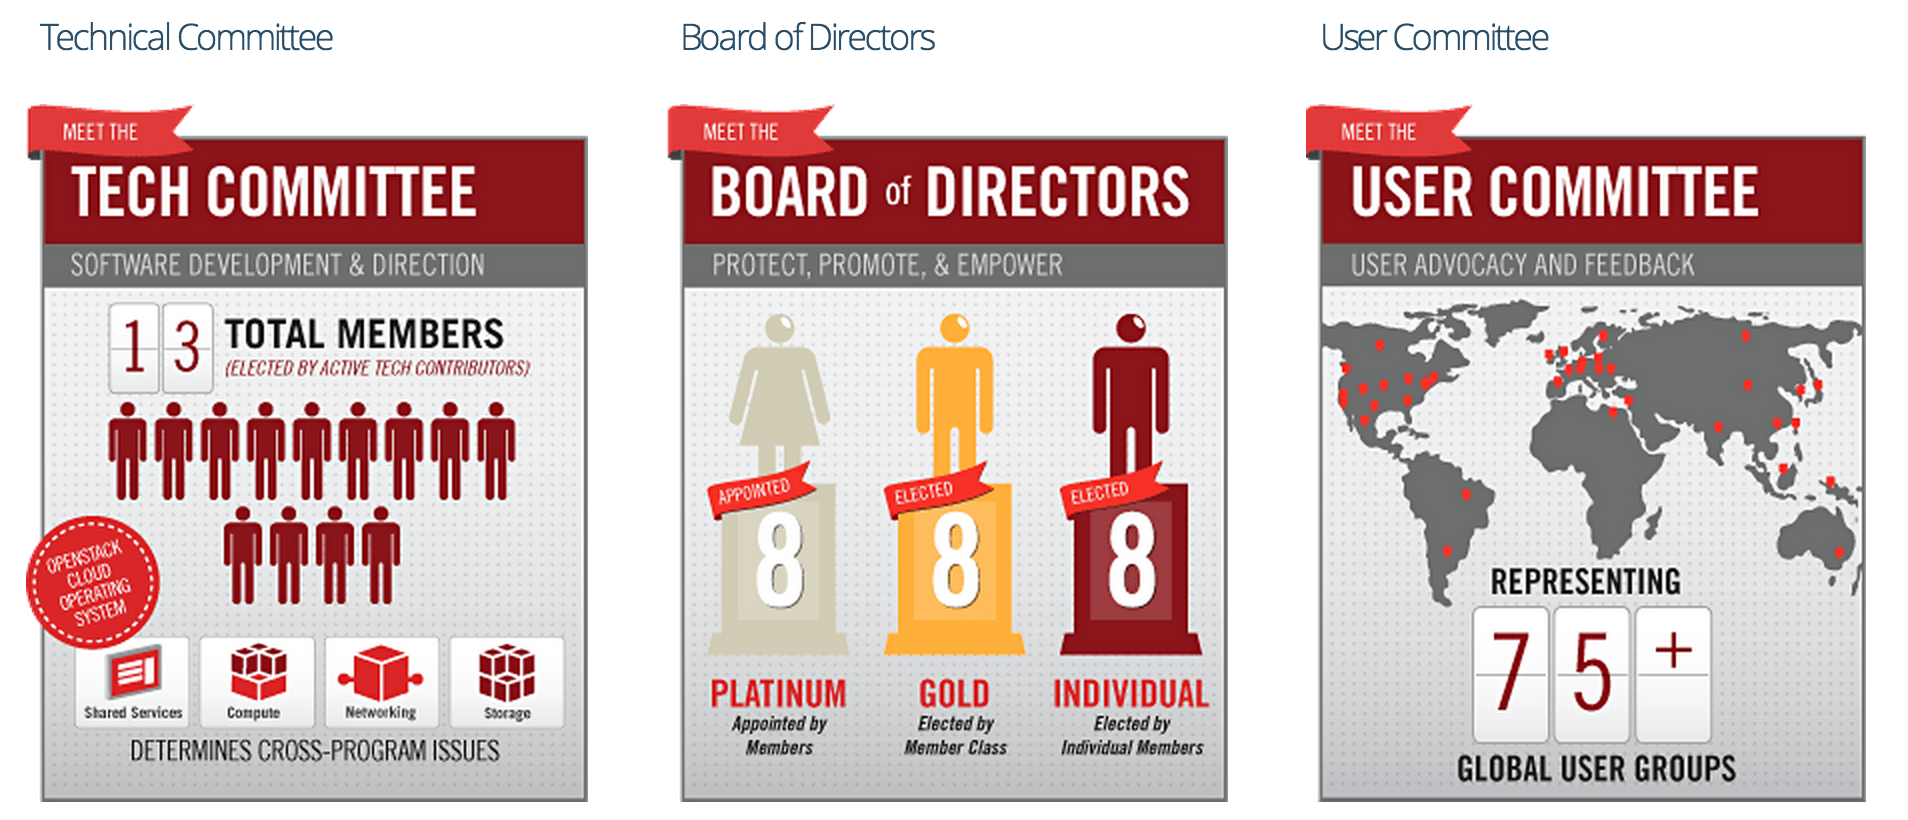
\includegraphics[width=\textwidth]{images/foundation.png}
  \end{frame}

  \begin{frame}
    \frametitle{Interface web / Dashboard : Horizon}
    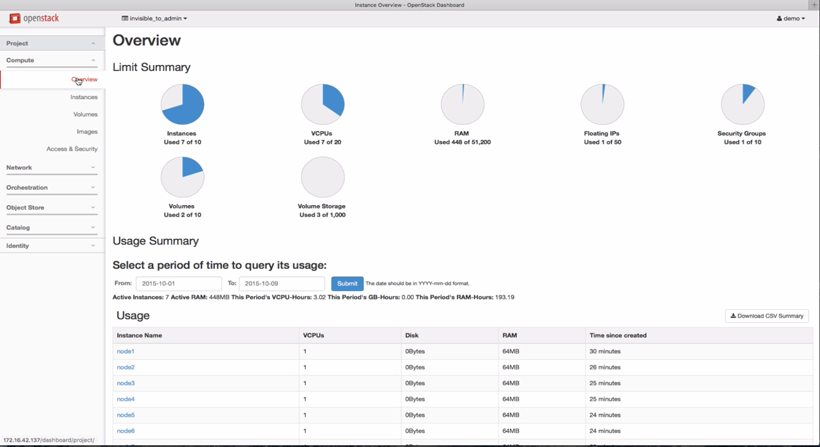
\includegraphics[width=\textwidth]{images/horizon.png}
  \end{frame}

  \begin{frame}
    \frametitle{Ressources}
    \begin{itemize}
      \item Annonces/sécurité : openstack-announce@lists.openstack.org
      \item Documentation : \url{http://docs.openstack.org/}
      \item Gouvernance du projet : \url{http://governance.openstack.org/}
      \item Support :
      \begin{itemize}
        \item \url{https://ask.openstack.org}
        \item openstack@lists.openstack.org
        \item \#openstack@Freenode
      \end{itemize}
      \item SDK/APIs : \url{http://developer.openstack.org/}
      \item Applications : \url{http://apps.openstack.org/}
      \item Actualités :
      \begin{itemize}
        \item Blog officiel : \url{http://www.openstack.org/blog/}
        \item Planet : \url{http://planet.openstack.org}
        \item Superuser : \url{http://superuser.openstack.org/}
        \item OpenStack Community Weekly Newsletter
      \end{itemize}
    \item Ressources commerciales : \url{http://www.openstack.org/marketplace/} entre autres
    \end{itemize}
  \end{frame}

  \begin{frame}
    \frametitle{Ressources - Communauté francophone}
    
\includegraphics{images/openstackfr.png}
    \begin{itemize}
      \item Site web : \url{http://openstack.fr/}
      \item Association des utilisateurs francophones d'OpenStack : \url{https://asso.openstack.fr/}
      \item Meetups : Paris, Rhônes-Alpes, Toulouse, Montréal, ...
      \item Présence à des événements tels que Solutions Linux
      \item Canaux de communication :
      \begin{itemize}
        \item openstack-fr@lists.openstack.org
        \item \#openstack-fr@Freenode
      \end{itemize}
    \end{itemize}
  \end{frame}
